%=============================================================================
%  Rapport hebdomadaire de stage -- Semaine 7
%  Projet : Simulateur de controleur aerien -- copilote IA pour le controle aerien
%  Auteur : Nicolas Marano -- URCA / supercalculateur ROMEO (NVIDIA GH200)
%  Compilation : pdflatex (x2 pour la table des matieres)
%=============================================================================
\documentclass[11pt,a4paper]{article}

\usepackage[utf8]{inputenc}
\usepackage[T1]{fontenc}
\usepackage[french]{babel}
\usepackage{lmodern}
\usepackage{microtype}
\usepackage[a4paper,margin=2.3cm,headheight=15pt]{geometry}
\usepackage{graphicx}
\usepackage{booktabs}
\usepackage{array}
\usepackage[table]{xcolor}
\usepackage{titlesec}
\usepackage{enumitem}
\usepackage{caption}
\usepackage{fancyhdr}
\usepackage{listings}
\usepackage[most]{tcolorbox}
\usepackage{hyperref}

%--- Couleurs ----------------------------------------------------------------
\definecolor{atcblue}{RGB}{11,61,145}
\definecolor{atcteal}{RGB}{13,110,124}
\definecolor{atcgreen}{RGB}{22,128,71}
\definecolor{atcred}{RGB}{197,32,38}
\definecolor{atcpurple}{RGB}{109,40,180}
\definecolor{atcslate}{RGB}{71,85,105}
\definecolor{lightgray}{RGB}{244,246,249}
\definecolor{rulegray}{RGB}{210,216,224}

\hypersetup{colorlinks=true, linkcolor=atcblue, urlcolor=atcteal, citecolor=atcblue,
  pdftitle={Rapport de stage -- Semaine 7}, pdfauthor={Nicolas Marano}}

%--- Titres ------------------------------------------------------------------
\titleformat{\section}{\Large\bfseries\color{atcblue}}{\thesection}{0.6em}{}
\titleformat{\subsection}{\large\bfseries\color{atcteal}}{\thesubsection}{0.6em}{}
\titleformat{\subsubsection}{\normalsize\bfseries\color{atcteal}}{\thesubsubsection}{0.5em}{}
\titlespacing*{\section}{0pt}{16pt}{8pt}

%--- En-tete / pied de page --------------------------------------------------
\pagestyle{fancy}
\fancyhf{}
\renewcommand{\headrulewidth}{0.4pt}
\renewcommand{\footrulewidth}{0.4pt}
\fancyhead[L]{\small\color{atcblue}\itshape Copilote IA pour le controle aerien}
\fancyhead[R]{\small\color{atcblue}\itshape Semaine 7}
\fancyfoot[L]{\small Nicolas Marano, URCA / ROMEO}
\fancyfoot[R]{\small\thepage}

%--- Boites tcolorbox --------------------------------------------------------
\newtcolorbox{objbox}{enhanced, colback=lightgray, colframe=atcblue,
  boxrule=0.8pt, arc=3pt, left=10pt, right=10pt, top=8pt, bottom=8pt,
  fonttitle=\bfseries\color{white}, coltitle=white, colbacktitle=atcblue,
  title={Objectif de la semaine}}

\newtcolorbox{resbox}{enhanced, colback=atcgreen!6, colframe=atcgreen,
  boxrule=0.8pt, arc=3pt, left=10pt, right=10pt, top=8pt, bottom=8pt,
  fonttitle=\bfseries, coltitle=white, colbacktitle=atcgreen,
  title={Resultats cles}}

\newtcolorbox{warnbox}{enhanced, colback=atcslate!6, colframe=atcslate,
  boxrule=0.8pt, arc=3pt, left=10pt, right=10pt, top=8pt, bottom=8pt,
  fonttitle=\bfseries, coltitle=white, colbacktitle=atcslate,
  title={Contraintes techniques et choix d'ingenierie}}

%--- Style des listings ------------------------------------------------------
\lstdefinestyle{atccode}{
  basicstyle=\ttfamily\footnotesize,
  backgroundcolor=\color{lightgray},
  frame=single, framesep=5pt, rulecolor=\color{rulegray},
  breaklines=true, breakatwhitespace=true,
  showstringspaces=false,
  keywordstyle=\color{atcblue}\bfseries,
  commentstyle=\color{atcgreen}\itshape,
  stringstyle=\color{atcpurple},
  numberstyle=\tiny\color{gray},
  columns=fullflexible, keepspaces=true,
  aboveskip=8pt, belowskip=8pt,
}
\lstset{style=atccode}

\setlist[itemize]{label=\textbullet, leftmargin=1.4em, itemsep=2pt, topsep=3pt}
\captionsetup{font=small, labelfont={bf,color=atcblue}}
\renewcommand{\arraystretch}{1.25}

%=============================================================================
\begin{document}

%--- Page de garde -----------------------------------------------------------
\begin{titlepage}
\centering
\vspace*{1.2cm}
{\color{atcblue}\rule{\textwidth}{2pt}}\\[0.5cm]
{\Huge\bfseries\color{atcblue} Rapport d'avancement de stage\par}
\vspace{0.35cm}
{\LARGE\color{atcteal} Semaine 7\par}
\vspace{0.25cm}
{\large Integration : une requete unifiee pour l'interpretation ancree \\[2pt]
(transcription + regles RAG + situation spatiale) vers un JSON exploitable\par}
\vspace{0.4cm}
{\color{atcblue}\rule{\textwidth}{2pt}}\\[1.0cm]

{\large\itshape Un copilote d'intelligence artificielle pour le controle aerien\par}
\vspace{1.6cm}

\begin{tabular}{rl}
\large\bfseries Auteur & \large Nicolas Marano\\[4pt]
\large\bfseries Projet & \large Simulateur de controleur aerien (PoC, 10 semaines)\\[4pt]
\large\bfseries Etablissement & \large Universite de Reims Champagne-Ardenne (URCA)\\[4pt]
\large\bfseries Calcul (IA) & \large Supercalculateur ROMEO : NVIDIA GH200 (Grace-Hopper, aarch64)\\[4pt]
\large\bfseries Domaine & \large Intelligence artificielle \& controle du trafic aerien\\[4pt]
\large\bfseries Periode & \large Semaine 7 du stage\\
\end{tabular}

\vfill
\begin{tcolorbox}[colback=lightgray, colframe=atcblue, arc=3pt, width=0.92\textwidth, center,
  left=12pt, right=12pt, top=8pt, bottom=8pt]
\small\centering
\textbf{Resume.} Cette semaine marque le debut de l'integration des modules
developpes separement. Une \emph{requete unifiee} est construite : elle assemble en
une seule entree la transcription de la clairance, les regles de phraseologie
recuperees par le RAG et une situation spatiale fixe (la topologie du secteur). Le
LLM produit en sortie un JSON conforme decrivant l'action a mener
(\texttt{\{callsign, action, value\}}). Une chaine de validation deterministe garantit
que ce JSON reste propre et exploitable : bornes physiques, fixes connus du secteur,
coherence semantique de l'instruction et presence de l'aeronef sur le radar.
\end{tcolorbox}
\vspace{0.6cm}
{\small Annee universitaire 2025--2026}
\end{titlepage}

%--- Table des matieres ------------------------------------------------------
\tableofcontents
\thispagestyle{fancy}
\vspace{1cm}

%=============================================================================
\section{Contexte et positionnement de la semaine}
%=============================================================================

Le projet automatise le dialogue radio pilote~/~controleur a l'interieur d'un
simulateur de trafic aerien. Une instruction parlee est transcrite, ancree dans la
phraseologie OACI, transformee en une commande validee, executee dans le simulateur
BlueSky, puis restituee en voix de pilote synthetisee. La chaine cible se resume
ainsi :

\begin{center}
\fbox{\parbox{0.95\textwidth}{\centering\ttfamily\footnotesize
voix pilote (VHF) $\rightarrow$ Whisper STT $\rightarrow$ NER + LLM avec RAG (OACI Doc 4444)
$\rightarrow$ JSON valide\\
$\rightarrow$ simulateur BlueSky (manoeuvre avion) $\rightarrow$ voix de readback synthetisee $\rightarrow$ boucle}}
\end{center}

Les semaines precedentes ont produit, et valide separement, le module de
\textbf{perception} (semaine~4), le module d'\textbf{interpretation} par RAG
(semaine~5) et le module de \textbf{restitution vocale} (semaine~6). La semaine~7
ouvre la phase d'\textbf{integration}. L'objectif est de reunir les entrees du module
d'interpretation au sein d'une \textbf{requete unifiee} : plutot que de traiter la
transcription isolement, le systeme la combine avec les regles de phraseologie
pertinentes et avec une representation de l'espace aerien, afin que le LLM dispose de
tout le contexte necessaire pour produire, en une passe, un JSON propre decrivant
l'action. A ce stade, la situation spatiale fournie est \textbf{fixe} (la topologie
statique du secteur) ; l'injection de l'etat de trafic en temps reel constitue
l'etape suivante.

\subsection{Synthese chiffree de la semaine}

\begin{table}[h]
\centering
\small
\begin{tabular}{>{\raggedright}p{8.7cm} l}
\toprule
\rowcolor{lightgray}\textbf{Indicateur} & \textbf{Resultat}\\
\midrule
Entrees combinees dans la requete unifiee & \textbf{3} (transcription, regles, espace)\\
Fixes de la situation spatiale (secteur) & 7\\
Segments / separation imposee & 6 / 5~NM\\
Plus court chemin \texttt{ENTRY\_W} $\rightarrow$ \texttt{EXIT\_E} & 101~NM\\
JSON exploitable produit (40 transcriptions reelles) & \textbf{100~\%}\\
Couches de validation du JSON de sortie & \textbf{4}\\
\bottomrule
\end{tabular}
\caption{Vue d'ensemble des resultats obtenus durant la semaine 7.}
\end{table}

%=============================================================================
\section{Semaine 7 : La requete unifiee}
%=============================================================================

\begin{objbox}
Construire une requete unifiee prenant en entree la transcription, les regles du RAG
et une situation spatiale fixe, et produisant en sortie un JSON propre et exploitable
decrivant l'action a mener (\texttt{\{callsign, action, value, [wpt]\}}).
\end{objbox}

\subsection{Les trois entrees de la requete}

La requete unifiee agrege trois sources d'information complementaires :

\begin{itemize}
  \item \textbf{La transcription} : le texte de la clairance, issu du module de
  reconnaissance vocale (semaine~4) ou saisi directement.
  \item \textbf{Les regles du RAG} : les fiches de phraseologie les plus pertinentes
  pour cette clairance, recuperees par recherche vectorielle (semaine~5, $k = 4$).
  \item \textbf{La situation spatiale fixe} : une representation de l'espace aerien
  (le graphe de secteur), qui fournit au LLM la liste des points connus et la
  topologie, et qui sert ensuite a valider les ordres de routage.
\end{itemize}

\subsection{La situation spatiale fixe : le graphe de secteur}

La situation spatiale est decrite par un graphe statique du secteur, charge depuis
\texttt{secteur\_graphe.json}. Il comporte 7~points (de type \emph{entry}, \emph{fix}
ou \emph{exit}), 6~segments orientes avec leur distance, et une separation imposee de
5~NM (figure~\ref{fig:graphe}). La classe \texttt{SectorGraph} expose la liste des
fixes, le voisinage, le plus court chemin (Dijkstra sur les distances) et un resume
textuel compact de la topologie. C'est ce resume qui est injecte dans la requete pour
donner au LLM une conscience spatiale, sans alourdir le \emph{prompt}.

\begin{lstlisting}[caption={Resume textuel de la topologie injecte dans la requete (\texttt{topology\_text()}).}]
Sector (separation 5.0 NM).
Fixes: ENTRY_W(entry), BALMO(fix), CROSS(fix), DELTA(fix), EXIT_E(exit), ENTRY_S(entry), NORTH(exit).
Segments: ENTRY_W-BALMO 25.0NM; BALMO-CROSS 25.5NM; CROSS-DELTA 25.5NM; CROSS-ENTRY_S 25.0NM; CROSS-NORTH 25.0NM; DELTA-EXIT_E 25.0NM.
\end{lstlisting}

\begin{figure}[h]
\centering
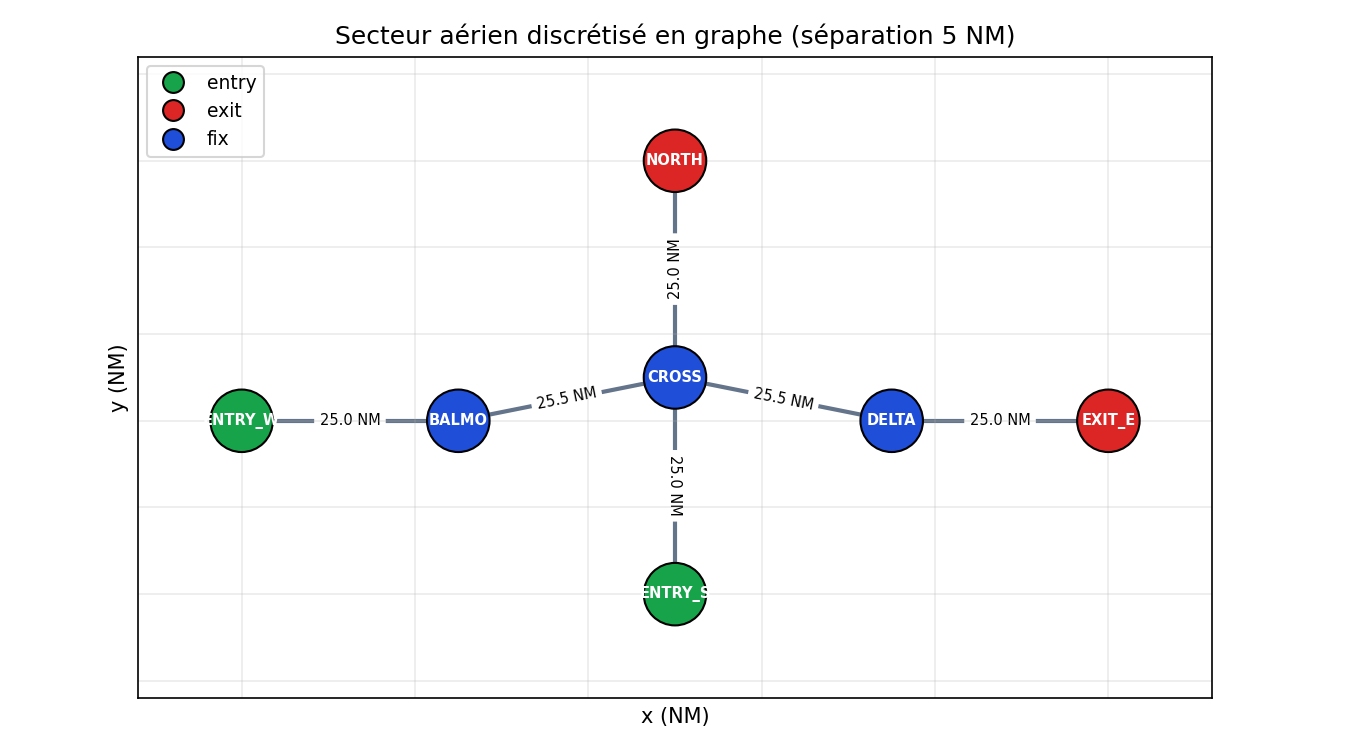
\includegraphics[width=0.66\textwidth]{figures/fig_secteur_graphe.png}
\caption{Situation spatiale fixe : le graphe du secteur (points d'entree, fixes,
sorties ; segments et distances). Il fournit le contexte spatial de la requete et
valide les ordres de routage. A ce stade, cette topologie est statique (sans etat de
trafic).}
\label{fig:graphe}
\end{figure}

\subsection{Construction de la requete unifiee}

La fonction \texttt{build\_messages} assemble les trois entrees en un unique message
adresse au LLM, precede d'un \emph{prompt} systeme strict qui impose une sortie au
format JSON et seulement cela. Les regles recuperees, la topologie du secteur, les
indices d'entites (indicatif, intentions) et la transcription sont concatenes dans un
ordre fixe.

\begin{lstlisting}[language=Python, caption={Assemblage de la requete unifiee (extrait de \texttt{atc\_llm.py}).}]
rules  = "\n".join(f"- {d['title']}: {d['text']}" for d, _ in retrieved)
sector = f"Sector graph: {graph.topology_text()}\n\n"
hint   = f"callsign={ner_callsign}; intentions_detectees={ner_intentions}"
user = (f"Applicable ICAO phraseology rules:\n{rules}\n\n"
        f"{sector}"
        f"NER hints: {hint}\n\n"
        f"Controller transcription: \"{transcription}\"\n\n"
        "Return ONLY the JSON array of orders.")
messages = [{"role": "system", "content": SYSTEM}, {"role": "user", "content": user}]
\end{lstlisting}

Sur un exemple, la requete assemblee et la sortie attendue prennent la forme
suivante :

\begin{lstlisting}[caption={Requete unifiee assemblee (abregee) et JSON produit par le LLM.}]
Applicable ICAO phraseology rules:
- Instruction de cap (heading): ... action HDG, value = cap en degres ...

Sector graph: Sector (separation 5.0 NM). Fixes: ENTRY_W(entry), BALMO(fix), ...

NER hints: callsign=AFR1234; intentions_detectees=['turn']

Controller transcription: "air france one two three four turn right heading two seven zero"

Return ONLY the JSON array of orders.
-->  [{"callsign": "AFR1234", "action": "HDG", "value": 270}]
\end{lstlisting}

\subsection{Orchestration : de la transcription au JSON}

La fonction \texttt{interpret()} enchaine les etapes de la requete unifiee :
extraction des entites (NER) pour l'indicatif et les intentions, recuperation des
$k = 4$ fiches pertinentes, assemblage de la requete, generation par le LLM
(Mistral~7B), puis analyse tolerante du JSON et validation. La sortie est une liste
d'ordres structures, chacun associe a sa traduction executable ou a un motif de rejet.

\subsection{Garantir un JSON propre et exploitable}

L'integration ne se limite pas a produire du JSON : elle doit produire du JSON
\emph{exploitable sans risque}. Quatre verifications deterministes s'appliquent en
aval de la generation.

\begin{enumerate}[label=\textbf{\arabic*.}, leftmargin=2.0em]
  \item \textbf{Schema et bornes} : chaque ordre est traduit par
  \texttt{json\_to\_trafscript} ; toute valeur hors bornes (HDG 0--360, ALT
  0--45000, SPD 0--350) ou action inconnue est rejetee.
  \item \textbf{Coherence spatiale} : un ordre de routage (\texttt{ADDWPT}) doit
  cibler un fix \emph{connu} du secteur, sinon il est rejete ou normalise vers le fix
  correct.
  \item \textbf{Coherence semantique} : si la clairance dit ``descend'' (sans
  ``climb'') mais que l'ordre vise un niveau \emph{au-dessus} du niveau actuel de
  l'aeronef, l'ordre est juge incoherent (transcription tronquee ou hallucination) et
  rejete plutot qu'execute ; le critere est symetrique pour ``climb''.
  \item \textbf{Realisme radio} : un ordre adresse a un indicatif absent du radar ne
  produit aucune reponse et n'est pas transmis au simulateur.
\end{enumerate}

\begin{warnbox}
A ce stade de l'integration, la situation spatiale fournie au LLM est volontairement
\emph{statique} : seule la topologie du secteur est injectee, pas encore l'etat de
trafic (positions et niveaux des aeronefs), qui fera l'objet de l'etape suivante. La
topologie est transmise sous forme d'un resume textuel compact plutot que du JSON
complet du graphe, afin de limiter la taille de la requete et de ne pas diluer
l'instruction. Le \emph{prompt} systeme reste strict pour que l'ajout du bloc spatial
ne pousse pas le modele a commenter sa reponse : seule la liste JSON est demandee, et
une analyse tolerante recupere le tableau meme si le modele ajoute du texte. La
verification de coherence semantique requiert l'altitude courante de l'aeronef ; elle
s'applique donc au moment de l'execution, lorsque cet etat est disponible.
\end{warnbox}

\subsection{Resultats et mesures}

\begin{resbox}
\begin{itemize}
  \item \textbf{Requete unifiee} operationnelle : transcription, regles RAG et
  situation spatiale fixe combinees en une seule passe vers le LLM.
  \item \textbf{JSON exploitable} produit sur 40 transcriptions reelles : 100~\%.
  \item \textbf{Validation de routage} : un \texttt{ADDWPT} vers un fix connu
  (\texttt{BALMO}) est accepte ; vers un point inconnu (\texttt{tango bravo}), il est
  rejete.
  \item \textbf{Garde-fou semantique} : une clairance tronquee de type ``descend
  flight level one'' qui ferait monter l'aeronef est detectee et rejetee.
\end{itemize}
\end{resbox}

\noindent\textbf{Analyse.} La requete unifiee atteint son objectif : sur les
transcriptions reelles evaluees, la sortie est systematiquement un JSON analysable, et
les quatre couches de validation eliminent les ordres dangereux, mal route ou
semantiquement incoherents avant toute execution. L'apport de l'integration ne tient
pas seulement a l'ajout du contexte spatial, mais aussi a la \emph{convergence} des
verifications en un point unique : un meme ordre est confronte aux bornes physiques,
a la topologie du secteur et a la coherence de l'instruction. La principale limite a
ce stade est que la conscience spatiale du LLM reste statique : il connait la
geometrie du secteur mais pas la position courante des aeronefs. C'est cette derniere
information qui permettra, ensuite, des decisions reellement situees (anticipation de
conflit, routage tenant compte du trafic).

%=============================================================================
\section{Bilan et transition}
%=============================================================================

La semaine~7 etablit le socle de l'integration : une requete unifiee qui combine la
transcription, les regles du RAG et une situation spatiale fixe, et dont la sortie est
un JSON propre et exploitable decrivant l'action a mener. La fiabilite de cette sortie
repose sur quatre verifications deterministes appliquees en aval du LLM (bornes,
coherence spatiale, coherence semantique, presence au radar).

\medskip
\noindent\textbf{Prochaines etapes.} L'etape directe consiste a remplacer la situation
spatiale \emph{fixe} par l'etat de trafic \emph{courant} (positions, caps et niveaux
des aeronefs lus dans le simulateur), afin de passer d'une conscience spatiale
statique a une conscience situee. Suivront la consolidation de la boucle temps reel
de bout en bout et une evaluation quantitative sur des scenarios complets.

\vfill
\begin{center}
\small\color{atcblue}\rule{0.5\textwidth}{0.6pt}\\[4pt]
\textit{Rapport d'avancement, Semaine 7, Nicolas Marano}\\
\textit{Stage : copilote IA pour le controle aerien, URCA / supercalculateur ROMEO}
\end{center}

\end{document}
